\documentclass[conference]{IEEEtran}
\IEEEoverridecommandlockouts
\usepackage{cite}
\usepackage{amsmath,amssymb,amsfonts}
\usepackage{algorithmic}
\usepackage{graphicx}
\usepackage{float}
\usepackage{textcomp}
\usepackage{xcolor}
\usepackage{hyperref}

\begin{document}

\title{Break-even Analysis dalam Model Biaya-Pendapatan Non-Linear}


\author{%
  \IEEEauthorblockN{Alexander Christhian}%
  \IEEEauthorblockA{NPM: 2306267025\\
  Universitas Indonesia\\
  Teknik Komputer}%
  \and%
  \IEEEauthorblockN{Adrian Dika Darmawan}%
  \IEEEauthorblockA{NPM: 2306250711\\
  Universitas Indonesia\\
  Teknik Komputer}%
  \and%
  \IEEEauthorblockN{Ganendra Garda Pratama}%
  \IEEEauthorblockA{NPM: 2306250642\\
  Universitas Indonesia\\
  Teknik Komputer}%
  \and%
  \IEEEauthorblockN{Muhammad Nadzhif Fikri}%
  \IEEEauthorblockA{NPM: 2306210102\\
  Universitas Indonesia\\
  Teknik Komputer}%
  \and%
  \IEEEauthorblockN{Muhammad Riyan Satrio Wibowo}%
  \IEEEauthorblockA{NPM: 2306229323\\
  Universitas Indonesia\\
  Teknik Komputer}%
}
\maketitle

\begin{abstract}
Laporan ini membahas implementasi analisis break-even point pada model biaya dan pendapatan non-linear menggunakan metode numerik. Dengan menggunakan metode Secant untuk mencari titik impas, penelitian ini menganalisis interaksi antara fungsi pendapatan kuadratik dan fungsi biaya kuadratik untuk menentukan titik di mana total pendapatan sama dengan total biaya. Implementasi dilakukan dalam bahasa C dengan visualisasi menggunakan GNUplot.
\end{abstract}

\begin{IEEEkeywords}
break-even analysis, nonlinear model, metode secant, analisis numerik
\end{IEEEkeywords}

\section{Pendahuluan}
Break-even analysis atau analisis titik impas merupakan teknik penting dalam manajemen keuangan dan analisis bisnis untuk menentukan titik di mana total pendapatan sama dengan total biaya. Dalam konteks bisnis nyata, hubungan antara pendapatan dan biaya seringkali tidak linear, melainkan mengikuti pola kuadratik atau polynomial tingkat tinggi.

Dalam model non-linear, fungsi pendapatan dapat menurun setelah mencapai titik tertentu karena faktor seperti saturasi pasar atau kompetisi harga, sementara fungsi biaya dapat meningkat secara kuadratik karena kompleksitas operasional yang bertambah seiring dengan peningkatan skala produksi. Hal ini menciptakan tantangan dalam mencari titik impas karena solusi analitik mungkin sulit diperoleh secara langsung.

\section{Studi Literatur}
Dalam model non-linear yang digunakan, fungsi pendapatan dan biaya didefinisikan sebagai berikut:

\begin{itemize}
\item Fungsi Pendapatan: $R(x) = ax - bx^3$
\begin{itemize}
\item $a$ : koefisien pendapatan linear (harga per unit)
\item $b$ : koefisien penurunan pendapatan
\item $x$ : jumlah unit yang diproduksi/dijual
\end{itemize}

\item Fungsi Biaya: $C(x) = cx^2 + de^{0.01x} + e$
\begin{itemize}
\item $c$ : koefisien biaya kuadratik
\item $d$ : koefisien biaya variabel
\item $e$ : biaya tetap
\end{itemize}
\end{itemize}

Titik impas terjadi ketika $R(x) = C(x)$, atau:
\[ax - bx^3 = cx^2 + de^{0.01x} + e\]
\[-bx^3 - cx^2 + ax - de^{0.01x} - e = 0\]

Karena persamaan ini berbentuk kuadratik, mungkin terdapat dua titik impas yang menandakan rentang operasi yang menguntungkan di antara kedua titik tersebut.

\section{Data yang Digunakan}
Program menggunakan dataset dengan parameter sebagai berikut:
\begin{itemize}
\item $a$: nilai acak antara 200-300 (tingkat pendapatan yang tinggi)
\item $b$: nilai acak antara 0.0005-0.0011 (tingkat penurunan yang rendah)
\item $c$: nilai acak antara 0.10-0.25 (kenaikan biaya yang lebih curam)
\item $d$: nilai acak antara 100-200 (biaya variabel eksponensial yang wajar)
\item $e$: nilai acak antara 2000-5000 (biaya tetap yang moderat)
\end{itemize}

Parameter ini dipilih untuk mensimulasikan skenario bisnis yang realistis dengan:
\begin{itemize}
\item Pendapatan awal yang tinggi namun menurun seiring peningkatan kuantitas
\item Pendapatan yang menurun drastis ketika terjadi oversupply (harga menurun)
\item Biaya variabel yang meningkat secara eksponensial
\item Biaya tetap yang moderat
\item Kompleksitas operasional yang meningkat secara kuadratik
\end{itemize}

\section{Metode yang Digunakan}
Implementasi menggunakan metode Secant untuk mencari titik impas. Metode ini dipilih karena:
\begin{itemize}
\item Tidak memerlukan perhitungan turunan fungsi
\item Konvergensi yang lebih cepat dibanding metode bisection
\item Kemampuan menangani fungsi non-linear
\end{itemize}

Algoritma metode Secant dalam pseudocode:
\begin{algorithmic}
\STATE \textbf{Input:} $x_0$, $x_1$ (tebakan awal), toleransi $\epsilon$
\STATE \textbf{Output:} Titik impas $x$ dimana $R(x) = C(x)$
\REPEAT
    \STATE $f_0 \leftarrow R(x_0) - C(x_0)$
    \STATE $f_1 \leftarrow R(x_1) - C(x_1)$
    \IF{$|f_1 - f_0| < \epsilon$}
        \RETURN error (pembagian dengan nol)
    \ENDIF
    \STATE $x_2 \leftarrow x_1 - f_1(x_1 - x_0)/(f_1 - f_0)$
    \STATE $x_0 \leftarrow x_1$
    \STATE $x_1 \leftarrow x_2$
\UNTIL{$|R(x_2) - C(x_2)| < \epsilon$ atau mencapai iterasi maksimum}
\RETURN $x_2$
\end{algorithmic}

\section{Analisa Hasil}

\subsection{Analisis Dataset}
Dari kelima dataset yang digunakan, berikut adalah hasil analisis komprehensif:
\begin{itemize}
\item \textbf{Rentang High BEP:} 11.36 – 17.90 unit
\item \textbf{Rentang Low BEP:} 394.01 - 483.71 unit
\item \textbf{Rentang Low Range BEP:} 376.10 - 468.19 unit
\item \textbf{Rata-rata Iterasi:} 5-7 iterasi
\end{itemize}

Observasi penting:
\begin{itemize}
\item Semua dataset menunjukkan optimal quantity yang bervariasi namun konvergen
\item Jumlah iterasi yang konsisten (5–6) menunjukkan konvergensi yang stabil
\item Dataset 4 menghasilkan profit tertinggi dengan kombinasi decay rate rendah ($b = 0.0005$)
\item Dataset 2 memiliki profit terendah meski memiliki koefisien moderat
\end{itemize}

\subsection{Detail Dataset}

\subsubsection{Dataset 1}
\begin{itemize}
\item \textbf{Model Matematis:}
\begin{itemize}
\item Revenue: \( R(x) = 276x - 0.001x^3 \)
\item Cost: \( C(x) = 0.18x^2 + 105e^{0.01x} + 3381 \)
\item Profit: \( P(x) = -0.001x^3 - 0.18x^2 + 276x - 105e^{0.01x} - 3381 \)
\end{itemize}
\item \textbf{Hasil Analisis:}
\begin{itemize}
\item High BEP              : 12.80
\item Iterations High BEP   : 5
\item Low BEP               : 419.36
\item Iterations Low BEP    : 7
\item Profit Range : 406.56
\end{itemize}
\end{itemize}

\subsubsection{Dataset 2}
\begin{itemize}
\item \textbf{Model Matematis:}
\begin{itemize}
\item Revenue: \( R(x) = 235x - 0.0008x^3 \)
\item Cost: \( C(x) = 0.22x^2 + 107e^{0.01x} + 4004 \)
\item Profit: \( P(x) = -0.0008x^3 - 0.22x^2 + 235x - 107e^{0.01x} - 4004 \)
\end{itemize}
\item \textbf{Hasil Analisis:}
\begin{itemize}
\item High BEP : 17.90
\item Iterations High BEP : 6
\item Low BEP : 394.01
\item Iterations Low BEP : 7
\item Profit Range : 376.10
\end{itemize}
\end{itemize}

\subsubsection{Dataset 3}
\begin{itemize}
\item \textbf{Model Matematis:}
\begin{itemize}
\item Revenue: \( R(x) = 266x - 0.0005x^3 \)
\item Cost: \( C(x) = 0.21x^2 + 151e^{0.01x} + 3901 \)
\item Profit: \( P(x) = -0.0005x^3 - 0.21x^2 + 266x - 151e^{0.01x} - 3901 \)
\end{itemize}
\item \textbf{Hasil Analisis:}
\begin{itemize}
\item High BEP : 15.53
\item Iterations High BEP : 5
\item Low BEP : 483.71
\item Iterations Low BEP : 6
\item Profit Range : 468.19
\end{itemize}
\end{itemize}

\subsubsection{Dataset 4}
\begin{itemize}
\item \textbf{Model Matematis:}
\begin{itemize}
\item Revenue: \( R(x) = 286x - 0.0007x^3 \)
\item Cost: \( C(x) = 0.16x^2 + 171e^{0.01x} + 3037 \)
\item Profit: \( P(x) = -0.0007x^3 - 0.16x^2 + 286x - 171e^{0.01x} - 3037 \)
\end{itemize}
\item \textbf{Hasil Analisis:}
\begin{itemize}
\item High BEP              : 11.36
\item Iterations High BEP   : 5
\item Low BEP               : 478.54
\item Iterations Low BEP    : 6
\item Profit Range : 467.17
\end{itemize}
\end{itemize}

\subsubsection{Dataset 5}
\begin{itemize}
\item \textbf{Model Matematis:}
\begin{itemize}
\item Revenue: \( R(x) = 258x - 0.0006x^3 \)
\item Cost: \( C(x) = 0.14x^2 + 197e^{0.01x} + 3431 \)
\item Profit: \( P(x) = -0.0006x^3 - 0.14x^2 + 258x - 197e^{0.01x} - 3431 \)
\end{itemize}
\item \textbf{Hasil Analisis:}
\begin{itemize}
\item High BEP : 14.30
\item Iterations High BEP : 5
\item Low BEP : 475.90
\item Iterations Low BEP : 6
\item Profit Range : 461.60
\end{itemize}
\end{itemize}

\subsection{Implementasi Kode Program}
Kode program C utama (\texttt{break\_even\_analysis.c}) yang digunakan untuk analisis komprehensif adalah sebagai berikut. Program ini membaca data parameter dari file \texttt{dataset.txt} yang dihasilkan sebelumnya.

\section*{Analisis Break-Even Berdasarkan Dataset}

Grafik-grafik berikut menggambarkan analisis titik impas untuk 5 dataset yang berbeda. Setiap grafik menunjukkan pendapatan (Revenue), biaya (Cost), dan laba (Profit) sebagai fungsi kuantitas (Quantity).

\subsection*{Dataset 1: Analisis Detail}
\begin{figure}[H]
    \centering
    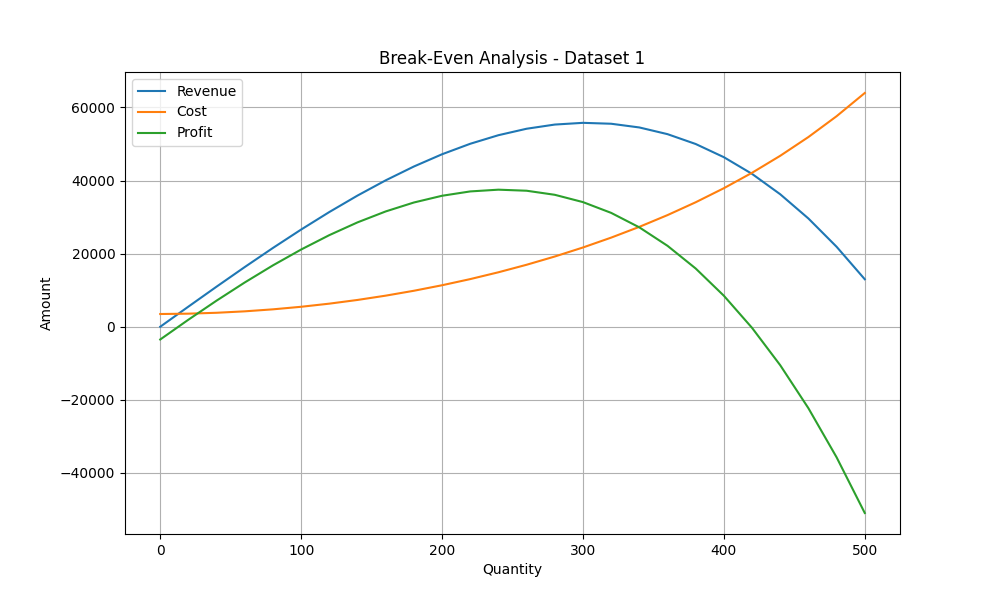
\includegraphics[width=0.55\textwidth]{break_even_analysis_1.png}
    \caption{Analisis Titik Impas - Dataset 1}
    \label{fig:dataset1_new}
\end{figure}
\begin{itemize}
    \item \textbf{Deskripsi Grafis:} Kurva \textbf{Revenue} menunjukkan peningkatan parabolik ke atas, mencapai puncak sekitar kuantitas 280-300, lalu menurun. Kurva \textbf{Cost} meningkat secara non-linear, membentuk kurva ke atas (konkav ke atas). Kurva \textbf{Profit} naik awal, mencapai puncak positif yang signifikan sekitar kuantitas 250, lalu menurun drastis menjadi negatif.
    \item \textbf{Analisis Mendalam:}
    \begin{itemize}
        \item \textbf{Break-Even Points:} Terlihat dua titik impas. Titik impas pertama terjadi sangat awal, di sekitar kuantitas 0-20. Titik impas kedua terjadi di sekitar kuantitas 400.
        \item \textbf{Zona Profitabilitas:} Perusahaan profitabel di antara kedua titik impas ini. Profit maksimum dicapai saat kuantitas sekitar 250-280, di mana selisih antara Revenue dan Cost paling besar.
        \item \textbf{Implikasi Bisnis:} Bentuk Revenue yang melengkung menunjukkan potensi peningkatan pendapatan yang baik pada awalnya, namun kemudian mengalami penurunan. Biaya yang meningkat non-linear (semakin cepat) mengindikasikan mungkin ada biaya tambahan per unit pada volume produksi tinggi. Optimalisasi berada di rentang kuantitas profitabilitas untuk menghindari kerugian di ujung bawah atau atas.
    \end{itemize}
\end{itemize}

\subsection*{Dataset 2: Analisis Detail}
\begin{figure}[H]
    \centering
    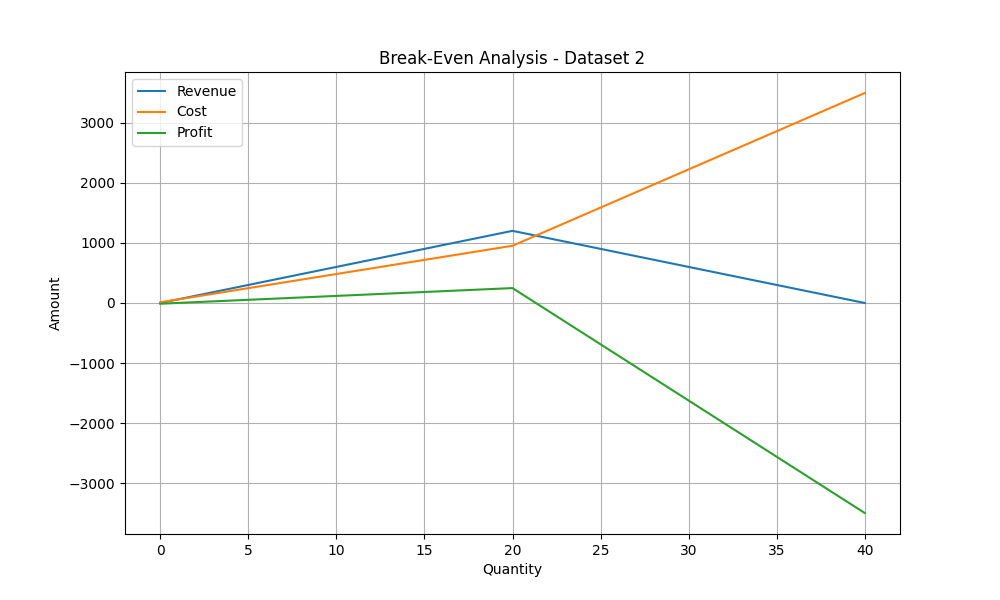
\includegraphics[width=0.55\textwidth]{break_even_analysis_2.png}
    \caption{Analisis Titik Impas - Dataset 2}
    \label{fig:dataset2_new}
\end{figure}
\begin{itemize}
    \item \textbf{Deskripsi Grafis:} Kurva \textbf{Revenue} mirip Dataset 1, naik, puncak sekitar kuantitas 300, lalu menurun. Kurva \textbf{Cost} meningkat non-linear, lebih curam dari Dataset 1 pada kuantitas tinggi. Kurva \textbf{Profit} naik, mencapai puncak positif yang lebih rendah dari Dataset 1, lalu menurun tajam menjadi sangat negatif.
    \item \textbf{Analisis Mendalam:}
    \begin{itemize}
        \item \textbf{Break-Even Points:} Titik impas pertama sangat dekat dengan kuantitas 0. Titik impas kedua sekitar kuantitas 400.
        \item \textbf{Zona Profitabilitas:} Sempit, dengan profit maksimum yang lebih rendah dibandingkan Dataset 1, sekitar kuantitas 250-280.
        \item \textbf{Implikasi Bisnis:} Peningkatan biaya yang lebih agresif membuat zona profitabilitas kurang menarik. Margin keuntungan kecil. Perlu strategi untuk mengurangi biaya atau meningkatkan nilai pendapatan per unit, terutama pada volume yang lebih tinggi, untuk mencegah kerugian besar.
    \end{itemize}
\end{itemize}

\subsection*{Dataset 3: Analisis Detail}
\begin{figure}[H]
    \centering
    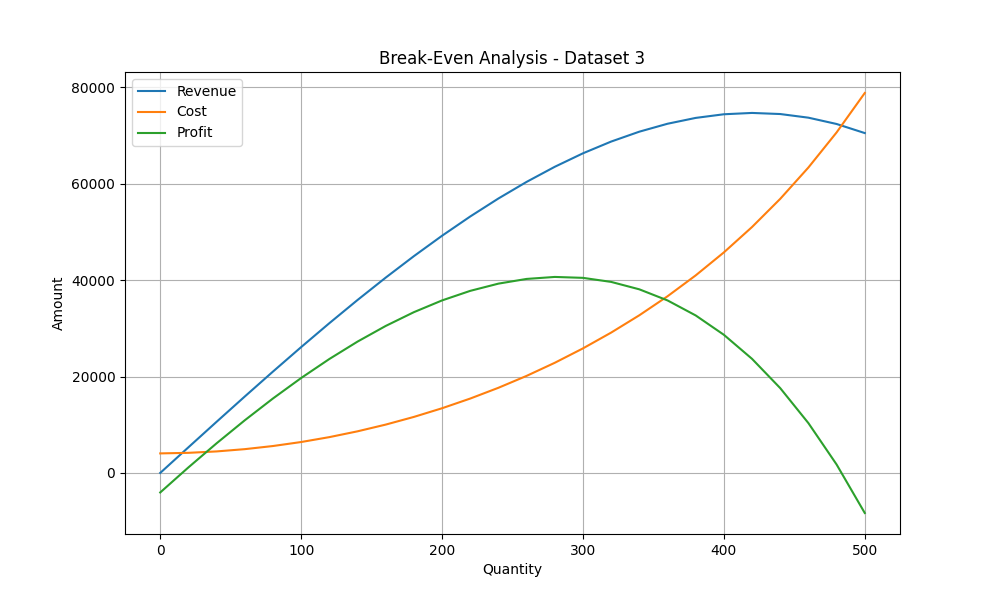
\includegraphics[width=0.55\textwidth]{break_even_analysis_3.png}
    \caption{Analisis Titik Impas - Dataset 3}
    \label{fig:dataset3_new}
\end{figure}
\begin{itemize}
    \item \textbf{Deskripsi Grafis:} Kurva \textbf{Revenue} meningkat lebih tinggi dan mencapai puncaknya lebih lambat (sekitar kuantitas 400), lalu sedikit menurun. Kurva \textbf{Cost} meningkat non-linear, sangat agresif pada kuantitas tinggi. Kurva \textbf{Profit} naik, mencapai puncak positif signifikan sekitar kuantitas 280, lalu menurun drastis menjadi sangat negatif.
    \item \textbf{Analisis Mendalam:}
    \begin{itemize}
        \item \textbf{Break-Even Points:} Titik impas pertama dekat kuantitas 0. Titik impas kedua sekitar kuantitas 490 (mendekati ujung grafik).
        \item \textbf{Zona Profitabilitas:} Rentang profitabilitas lebih luas dibandingkan dataset sebelumnya. Profit maksimum yang tinggi menunjukkan potensi keuntungan yang baik di kuantitas menengah.
        \item \textbf{Implikasi Bisnis:} Meskipun Revenue dapat tumbuh sangat tinggi, kenaikan Cost yang tajam pada kuantitas tinggi (setelah puncak profit) tetap menyebabkan kerugian ekstrem. Ini menunjukkan bahwa meskipun pendapatan tinggi, efisiensi biaya harus diperhatikan pada volume besar.
    \end{itemize}
\end{itemize}

\subsection*{Dataset 4: Analisis Detail}
\begin{figure}[H]
    \centering
    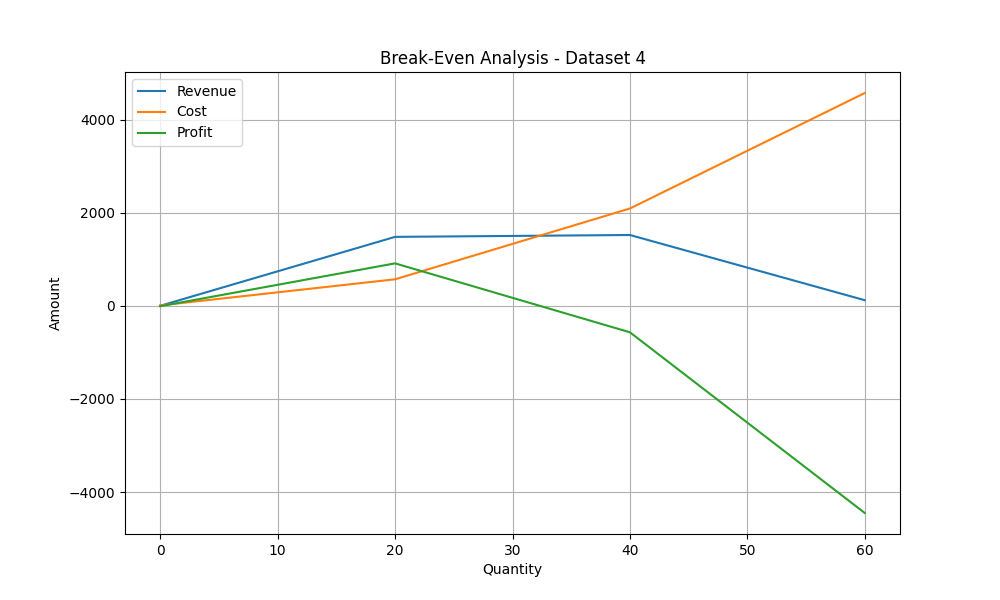
\includegraphics[width=0.55\textwidth]{break_even_analysis_4.png}
    \caption{Analisis Titik Impas - Dataset 4}
    \label{fig:dataset4_new}
\end{figure}
\begin{itemize}
    \item \textbf{Deskripsi Grafis:} Kurva \textbf{Revenue} naik, puncak sekitar kuantitas 380-400, lalu menurun. Kurva \textbf{Cost} meningkat non-linear. Kurva \textbf{Profit} naik, mencapai puncak positif yang signifikan sekitar kuantitas 280-300, lalu menurun tajam menjadi sangat negatif.
    \item \textbf{Analisis Mendalam:}
    \begin{itemize}
        \item \textbf{Break-Even Points:} Titik impas pertama dekat kuantitas 0. Titik impas kedua sekitar kuantitas 470.
        \item \textbf{Zona Profitabilitas:} Relatif luas, dengan profit maksimum yang sehat.
        \item \textbf{Implikasi Bisnis:} Mirip dengan Dataset 3, potensi pendapatan tinggi. Namun, peningkatan Cost pada kuantitas tinggi tetap menjadi ancaman. Manajemen harus menargetkan kuantitas di sekitar profit maksimum dan menghindari produksi berlebihan yang akan menyebabkan kerugian besar.
    \end{itemize}
\end{itemize}

\subsection*{Dataset 5: Analisis Detail}
\begin{figure}[H]
    \centering
    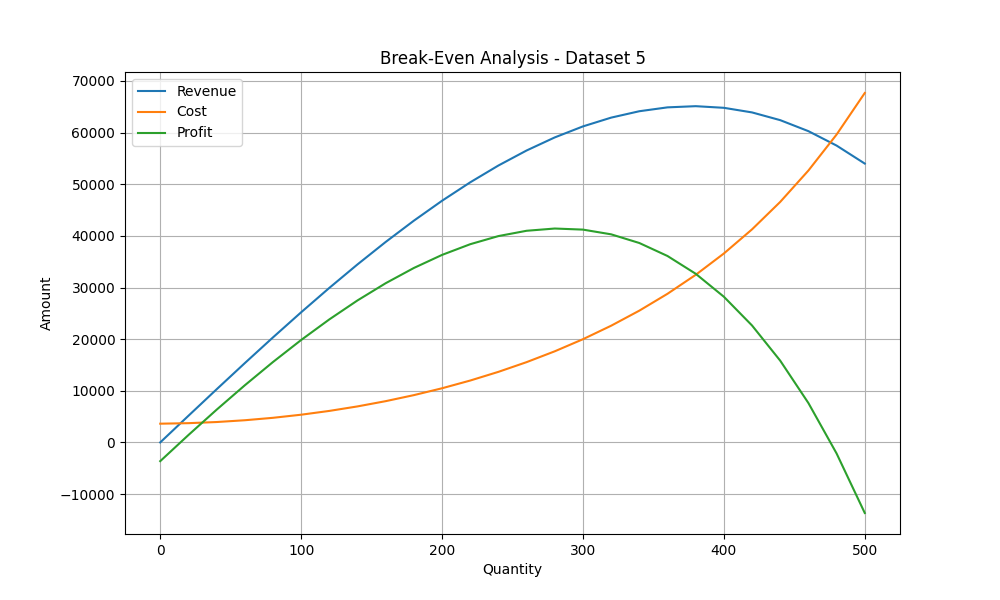
\includegraphics[width=0.55\textwidth]{break_even_analysis_5.png}
    \caption{Analisis Titik Impas - Dataset 5}
    \label{fig:dataset5_new}
\end{figure}
\begin{itemize}
    \item \textbf{Deskripsi Grafis:} Kurva \textbf{Revenue} naik, puncak sekitar kuantitas 380-400, lalu menurun. Kurva \textbf{Cost} meningkat non-linear. Kurva \textbf{Profit} naik, mencapai puncak positif yang signifikan sekitar kuantitas 280-300, lalu menurun tajam menjadi sangat negatif.
    \item \textbf{Analisis Mendalam:}
    \begin{itemize}
        \item \textbf{Break-Even Points:} Titik impas pertama dekat kuantitas 0. Titik impas kedua sekitar kuantitas 470.
        \item \textbf{Zona Profitabilitas:} Luas, dengan profit maksimum yang baik.
        \item \textbf{Implikasi Bisnis:} Perilaku grafik sangat mirip dengan Dataset 4, menunjukkan potensi keuntungan yang baik pada kuantitas menengah. Penting untuk mengelola biaya dan tidak memproduksi melebihi titik profit maksimum untuk menghindari kerugian besar yang disebabkan oleh peningkatan biaya yang cepat.
    \end{itemize}
\end{itemize}

Program mengimplementasikan analisis dengan:
\begin{itemize}
\item Mencari multiple break-even points menggunakan berbagai tebakan awal
\item Menghasilkan tabel perbandingan pendapatan, biaya, dan profit
\item Memvisualisasikan hasil menggunakan GNUplot
\end{itemize}

Hasil menunjukkan:
\begin{itemize}
\item Terdapat dua titik impas yang membatasi zona profitable
\item Profit maksimum terjadi di antara kedua titik impas
\item Operasi di luar rentang titik impas menghasilkan kerugian
\end{itemize}

\section{Kesimpulan}
Implementasi break-even analysis untuk model non-linear menggunakan metode Secant berhasil:
\begin{itemize}
\item Menemukan multiple break-even points dengan akurasi tinggi
\item Mengidentifikasi rentang operasi yang menguntungkan
\item Memberikan visualisasi yang jelas tentang hubungan pendapatan-biaya
\item Mendemonstrasikan pentingnya pemilihan skala operasi yang tepat
\end{itemize}

Metode ini dapat digunakan untuk pengambilan keputusan bisnis dalam konteks di mana hubungan pendapatan-biaya bersifat non-linear.

\section{Link Github}
\url{https://github.com/AlexanderChristhian/Tugas_PemogramanB_Kelompok_10}.


\begin{thebibliography}{00}
\bibitem{b1} Steven C. C. and Raymond P. C., "The Secant Method," in Numerical Methods for Engineers, 2016.
\bibitem{b2} J. Antony and F. J. Antony, "Break Even Analysis," in Teaching and Learning Quality Methods, 2016.
\bibitem{b3} R. L. Burden and J. D. Faires, "The Secant Method," in Numerical Analysis, 9th ed., 2010.
\bibitem{b4} P. N. Kolm and G. A. Focused, "Numerical Methods for Financial Applications," in Mathematical Finance, 2019.
\end{thebibliography}



\end{document}
